
\documentclass{article}
\usepackage{amstext}
\usepackage{amsfonts}
\usepackage{hyperref}
\usepackage[round]{natbib}
\usepackage{hyperref}
\usepackage{graphicx}
\usepackage{rotating}
%%\usepackage[nolists]{endfloat}
%%\usepackage{Sweave}

%%\VignetteIndexEntry{Survival Ensembles}
%%\VignetteDepends{mboost,ipred}

\newcommand{\Rpackage}[1]{{\normalfont\fontseries{b}\selectfont #1}}
\newcommand{\Robject}[1]{\texttt{#1}}
\newcommand{\Rclass}[1]{\textit{#1}}
\newcommand{\Rcmd}[1]{\texttt{#1}}
\newcommand{\Roperator}[1]{\texttt{#1}}
\newcommand{\Rarg}[1]{\texttt{#1}}
\newcommand{\Rlevel}[1]{\texttt{#1}}

\newcommand{\RR}{\textsf{R}}
\renewcommand{\S}{\textsf{S}}

\RequirePackage[T1]{fontenc}
\RequirePackage{graphicx,ae,fancyvrb}
\IfFileExists{upquote.sty}{\RequirePackage{upquote}}{}
\usepackage{relsize}

\DefineVerbatimEnvironment{Sinput}{Verbatim}{baselinestretch=1}
\DefineVerbatimEnvironment{Soutput}{Verbatim}{fontfamily=courier,
                                              baselinestretch=1,
                                              fontshape=it,
                                              fontsize=\relsize{-1}}
\DefineVerbatimEnvironment{Scode}{Verbatim}{}
\newenvironment{Schunk}{}{} 

\renewcommand{\baselinestretch}{1}

\hypersetup{%
  pdftitle = {mboost Illustrations},
  pdfsubject = {package vignette},
  pdfauthor = {Torsten Hothorn and Peter Buhlmann},
%% change colorlinks to false for pretty printing
  colorlinks = {true},
  linkcolor = {blue},
  citecolor = {blue},
  urlcolor = {red},
  hyperindex = {true},
  linktocpage = {true},
}

\begin{document}

\setkeys{Gin}{width=\textwidth}

\title{Survival Ensembles}

\author{Torsten Hothorn$^{1,\star}$, Peter B\"uhlmann$^2$, Sandrine Dudoit$^3$, \\
        Annette Molinaro$^4$ and Mark J. van der Laan$^3$}
\date{}
\maketitle

\noindent$^1$Institut f\"ur Medizininformatik, Biometrie und Epidemiologie\\
     Friedrich-Alexander-Universit\"at Erlangen-N\"urnberg\\
     Waldstra{\ss}e 6, D-91054 Erlangen, Germany \\
     Tel: ++49--9131--8522707 \\
     Fax: ++49--9131--8525740 \\
     \texttt{Torsten.Hothorn@R-project.org}
\newline

\noindent$^2$Seminar f\"ur Statistik, ETH Z\"urich,
             CH-8032 Z\"urich, Switzerland \\
            \texttt{buhlmann@stat.math.ethz.ch}
\newline

\noindent$^3$Division of Biostatistics, University of California, Berkeley \\
     140 Earl Warren Hall, \#7360, Berkeley, CA 94720-7360, USA \\
    \texttt{sandrine@stat.Berkeley.EDU} \\
    \texttt{laan@stat.Berkeley.EDU}
\newline

\noindent$^4$Division of Biostatistics, Epidemiology and Public Health\\
    Yale University School of Medicine, 206 LEPH \\
    60 College Street PO Box 208034, New Haven CT 06520-8034 \\
    \texttt{annette.molinaro@yale.edu}
\newline

\section{Illustrations and Applications}

This document reproduces the data analyses presented in
\cite{hothetal06}. For a description of the theory behind
applications shown here we refer to the original manuscript.

\subsection{Acute myeloid leukemia}


\paragraph{Data preprocessing}

Compute IPC weights, define risk score and set up learning sample:
\begin{Schunk}
\begin{Sinput}
R> AMLw <- IPCweights(Surv(clinical$time, clinical$event))
R> risk <- rep(0, nrow(clinical))
R> rlev <- levels(clinical[, "Cytogenetic.group"])
R> risk[clinical[, "Cytogenetic.group"] %in% rlev[c(7, 
         8, 4)]] <- "low"
R> risk[clinical[, "Cytogenetic.group"] %in% rlev[c(5, 
         9)]] <- "intermediate"
R> risk[clinical[, "Cytogenetic.group"] %in% rlev[-c(4, 
         5, 7, 8, 9)]] <- "high"
R> risk <- as.factor(risk)
R> AMLlearn <- cbind(clinical[, c("time", "Sex", 
         "Age", "LDH", "WBC", "FLT3.aberration.", "MLL.PTD", 
         "Tx.Group.")], risk = risk, iexpressions[, 
         colnames(iexpressions) %in% selgenes[["Clone.ID"]]])
R> cc <- complete.cases(AMLlearn)
R> AMLlearn <- AMLlearn[AMLw > 0 & cc, ]
R> AMLw <- AMLw[AMLw > 0 & cc]
\end{Sinput}
\end{Schunk}

\paragraph{Model fitting}

Fit random forest for censored data
\begin{Schunk}
\begin{Sinput}
R> ctrl <- cforest_control(mincriterion = 0.1, mtry = 5, 
         minsplit = 5, ntree = 250)
R> AMLrf <- cforest(I(log(time)) ~ ., data = AMLlearn, 
         control = ctrl, weights = AMLw)
\end{Sinput}
\end{Schunk}
and $L_2$Boosting for censored data
\begin{Schunk}
\begin{Sinput}
R> AMLl2b <- glmboost(I(log(time)) ~ ., data = AMLlearn, 
         weights = AMLw, control = boost_control(mstop = 5000))
\end{Sinput}
\end{Schunk}

\begin{figure}
\begin{center}
\begin{Schunk}
\begin{Sinput}
R> plot(aic <- AIC(AMLl2b))
\end{Sinput}
\end{Schunk}
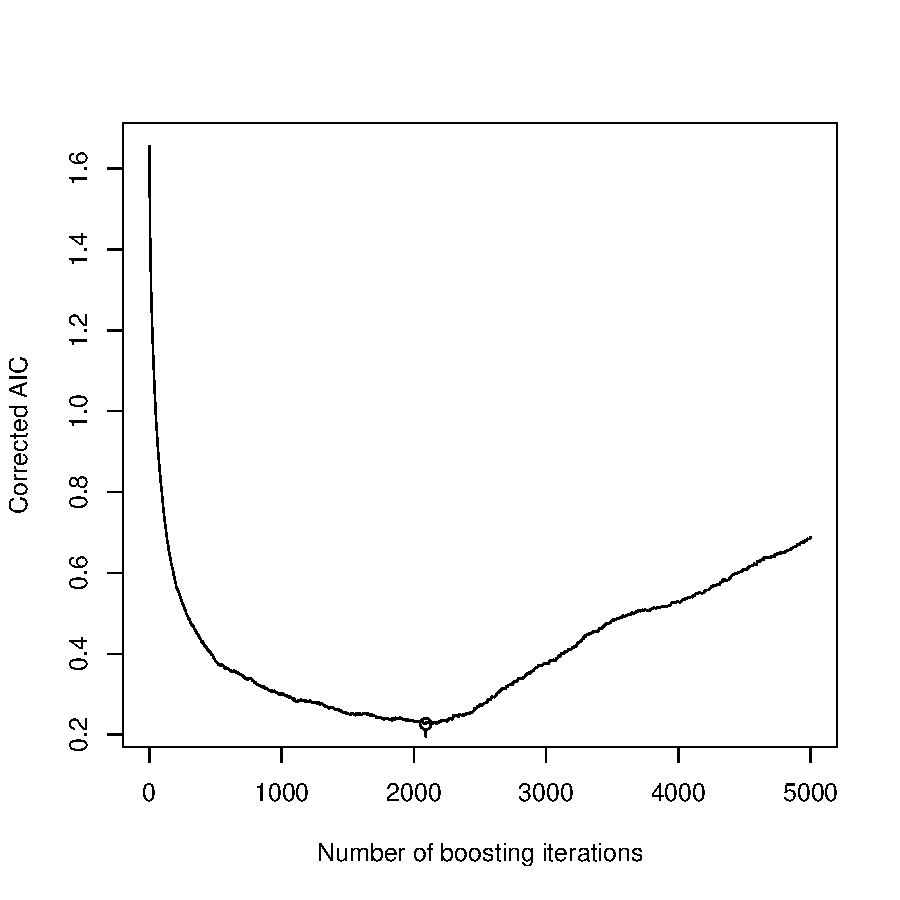
\includegraphics{SurvivalEnsembles-AML-AIC}
\caption{AIC criterion for AML data.}
\end{center}
\end{figure}

Compute fitted values
\begin{Schunk}
\begin{Sinput}
R> AMLl2b <- AMLl2b[mstop(aic)]
R> cAML <- coef(AMLl2b)
R> cAML[abs(cAML) > 0]
\end{Sinput}
\begin{Soutput}
     (Intercept)              Age              WBC 
      0.03094981       0.00854937      -0.00364371 
      MLL.PTDyes    Tx.Group.AUTO      Tx.Group.IC 
     -0.50709786       0.90185340       0.04037578 
    Tx.Group.Ind riskintermediate   `IMAGE:145643` 
     -1.86134842       0.11825619       0.19788355 
 `IMAGE:2542486`   `IMAGE:345601`   `IMAGE:377560` 
      0.00442375       0.02935101       0.11000322 
  `IMAGE:428782`  `IMAGE:2043415`  `IMAGE:1584563` 
      0.01010658       0.05911671      -0.17883619 
  `IMAGE:347035`   `IMAGE:262695`   `IMAGE:950479` 
     -0.03307600       0.00080156       0.09049309 
  `IMAGE:898305`  `IMAGE:1472689`   `IMAGE:150702` 
      0.00523016       0.03498572       0.01367553 
 `IMAGE:1526826`    `IMAGE:66507`   `IMAGE:786302` 
     -0.01805326       0.00399127       0.08941300 
  `IMAGE:243614`   `IMAGE:417884`  `IMAGE:1592006` 
     -0.05776062      -0.04890054      -0.02269622 
 `IMAGE:1917063`   `IMAGE:884333`   `IMAGE:133273` 
     -0.06536720       0.04189990       0.06594787 
  `IMAGE:950888`   `IMAGE:809533`    `IMAGE:49389` 
      0.02027810      -0.15986981       0.06352703 
  `IMAGE:789357`   `IMAGE:142139`  `IMAGE:1558053` 
     -0.01252187       0.00089307       0.07795515 
  `IMAGE:856174`   `IMAGE:504421`   `IMAGE:435036` 
      0.01115234       0.06861766       0.06094620 
  `IMAGE:491751`   `IMAGE:782835`    `IMAGE:52930` 
      0.04336285      -0.17924185      -0.03503330 
 `IMAGE:2545705`   `IMAGE:756405`   `IMAGE:502664` 
     -0.09886616       0.07713650       0.03620466 
  `IMAGE:129032`  `IMAGE:1610168`   `IMAGE:327676` 
     -0.31322459       0.01260374      -0.02117310 
   `IMAGE:69002`   `IMAGE:121551`  `IMAGE:2019101` 
     -0.41671336      -0.08107446      -0.06531175 
 `IMAGE:1456160`   `IMAGE:430318`  `IMAGE:2566064` 
     -0.10208684      -0.07297586       0.06126683 
   `IMAGE:74537`  `IMAGE:1606557`   `IMAGE:306812` 
      0.04523784       0.14243526       0.03504441 
  `IMAGE:565083`   `IMAGE:843028`    `IMAGE:68794` 
      0.29555347       0.05619983       0.23722775 
  `IMAGE:488505`   `IMAGE:167205`   `IMAGE:291756` 
      0.33464829       0.00217136       0.04973319 
  `IMAGE:810801`  `IMAGE:1702742`   `IMAGE:380462` 
      0.08725523      -0.04428190      -0.13182519 
  `IMAGE:154472`   `IMAGE:302540`   `IMAGE:135221` 
     -0.24723347       0.17175129      -0.01972168 
 `IMAGE:1567220`   `IMAGE:594630` 
      0.02473376      -0.07396882 
\end{Soutput}
\begin{Sinput}
R> AMLprf <- predict(AMLrf, newdata = AMLlearn)
R> AMLpb <- predict(AMLl2b, newdata = AMLlearn)
\end{Sinput}
\end{Schunk}

\begin{figure}
\begin{center}
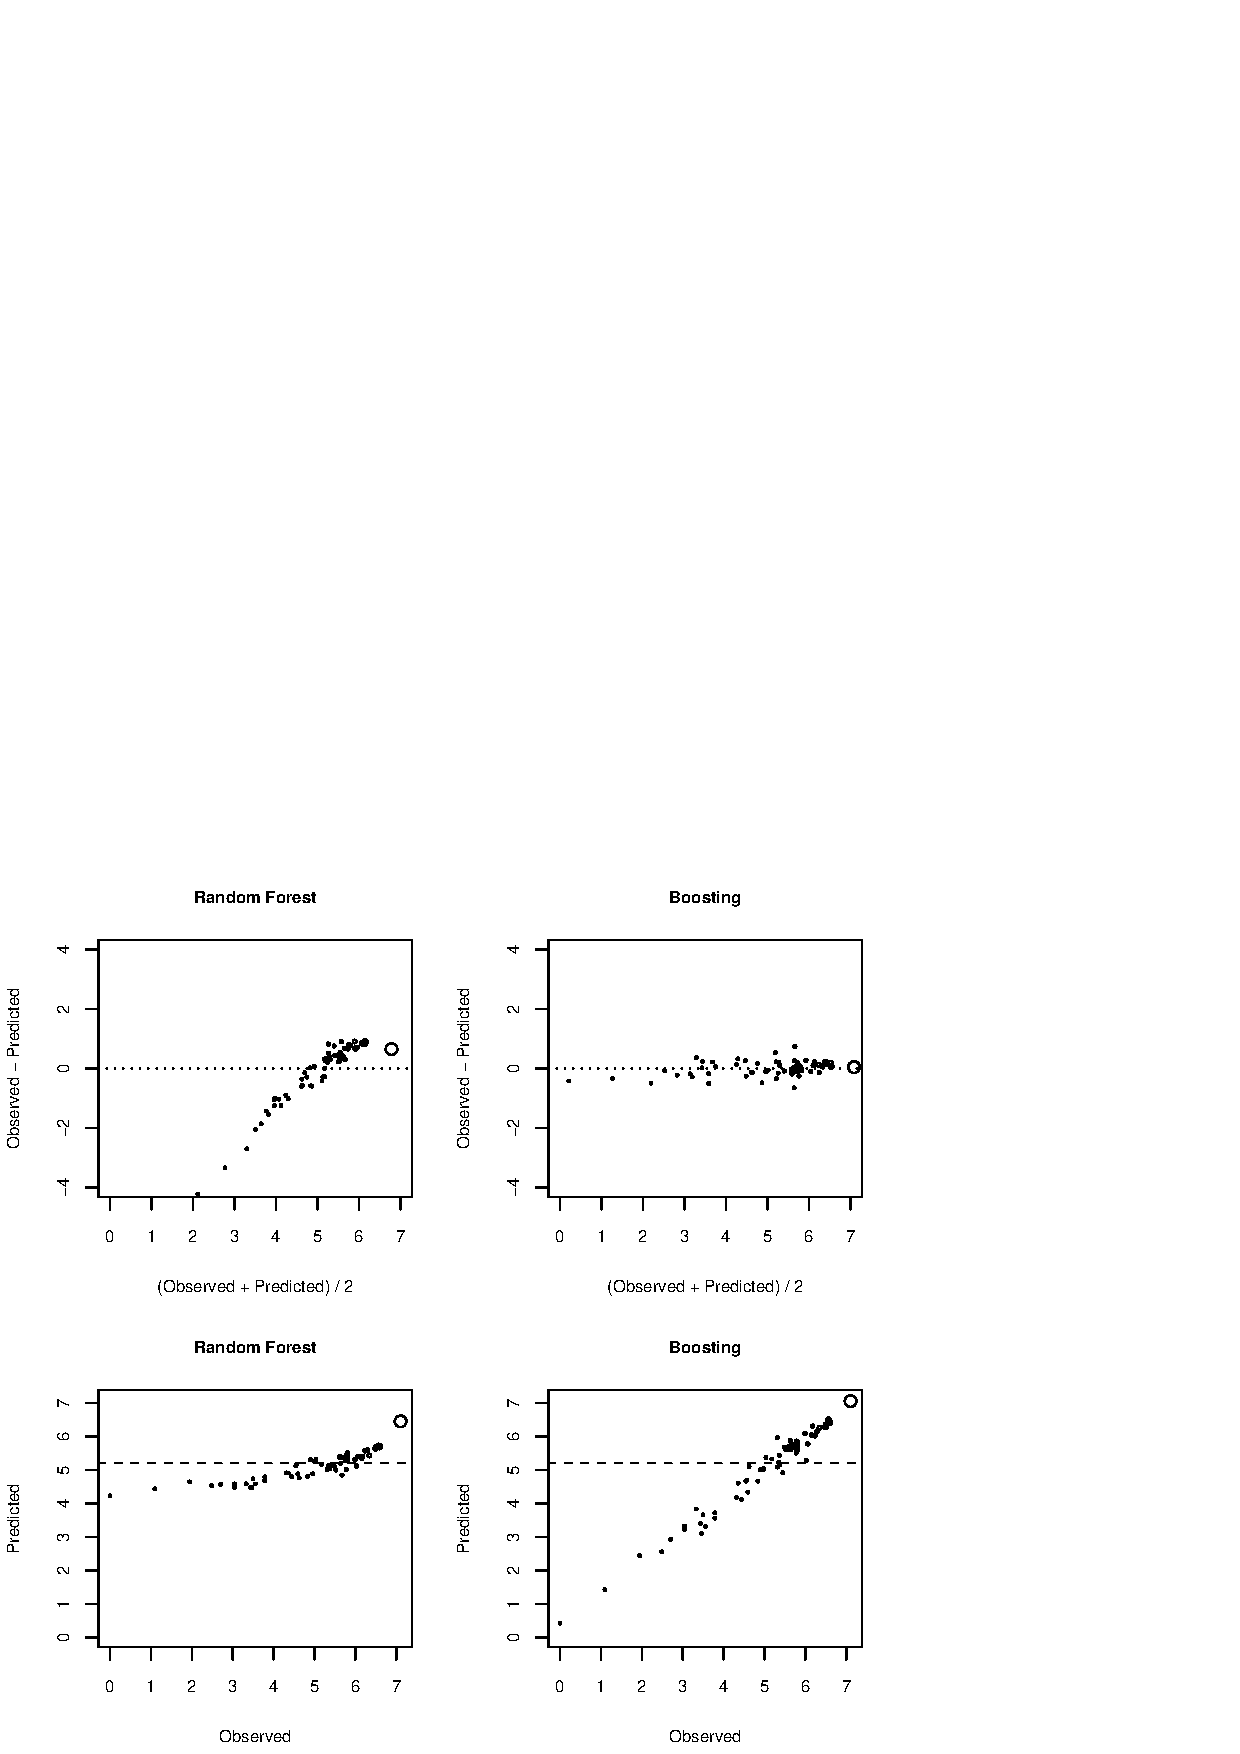
\includegraphics{SurvivalEnsembles-Figure1}
\caption{AML data: Reproduction of Figure 1.}
\end{center}
\end{figure}

\subsection{Node-positive breast cancer}

\paragraph{Data preprocessing}

Compute IPC weights and set up learning sample:
\begin{Schunk}
\begin{Sinput}
R> data("GBSG2", package = "ipred")
R> GBSG2w <- IPCweights(Surv(GBSG2$time, GBSG2$cens))
R> GBSG2learn <- cbind(GBSG2[, -which(names(GBSG2) %in% 
         c("time", "cens"))], ltime = log(GBSG2$time))
R> n <- nrow(GBSG2learn)
\end{Sinput}
\end{Schunk}

\paragraph{Model fitting}

\begin{Schunk}
\begin{Sinput}
R> LMmod <- lm(ltime ~ ., data = GBSG2learn, weights = GBSG2w)
R> LMerisk <- sum((GBSG2learn$ltime - predict(LMmod))^2 * 
         GBSG2w)/n
R> TRmod <- rpart(ltime ~ ., data = GBSG2learn, weights = GBSG2w)
R> TRerisk <- sum((GBSG2learn$ltime - predict(TRmod))^2 * 
         GBSG2w)/n
R> ctrl <- cforest_control(mincriterion = qnorm(0.95), 
         mtry = 5, minsplit = 5, ntree = 100)
R> RFmod <- cforest(ltime ~ ., data = GBSG2learn, 
         weights = GBSG2w, control = ctrl)
R> L2Bmod <- glmboost(ltime ~ ., data = GBSG2learn, 
         weights = GBSG2w, control = boost_control(mstop = 250))
R> L2BHubermod <- glmboost(ltime ~ ., data = GBSG2learn, 
         weights = GBSG2w, family = Huber(d = log(2)))
\end{Sinput}
\end{Schunk}

\begin{figure}
\begin{center}
\begin{Schunk}
\begin{Sinput}
R> plot(aic <- AIC(L2Bmod))
\end{Sinput}
\end{Schunk}
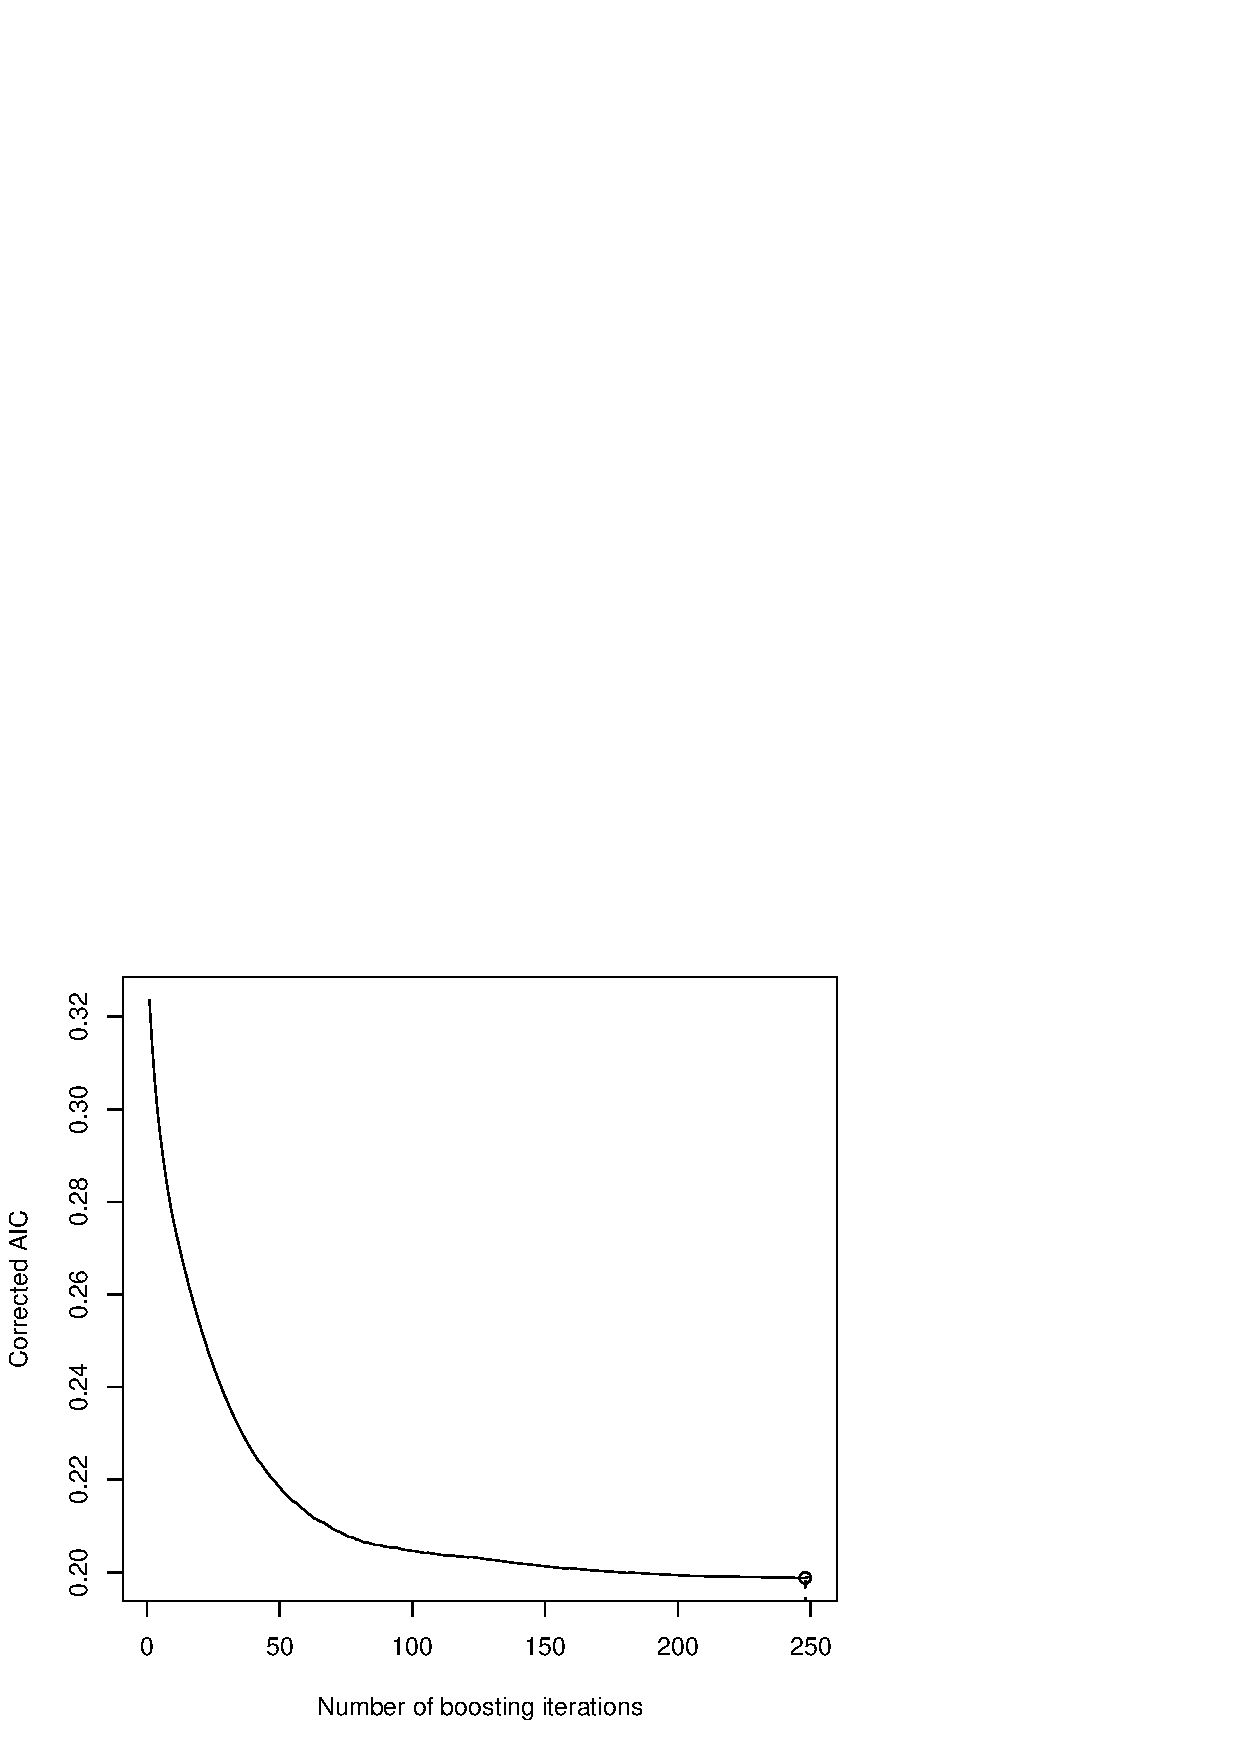
\includegraphics{SurvivalEnsembles-GBSG2-AIC}
\caption{AIC criterion for GBSG2 data.}
\end{center}
\end{figure}

Compute fitted values:
\begin{Schunk}
\begin{Sinput}
R> GBSG2Hp <- predict(L2BHubermod, newdata = GBSG2learn)
R> L2Berisk <- sum((GBSG2learn$ltime - predict(L2Bmod, 
         newdata = GBSG2learn))^2 * GBSG2w)/n
R> RFerisk <- sum((GBSG2learn$ltime - predict(RFmod, 
         newdata = GBSG2learn))^2 * GBSG2w)/n
\end{Sinput}
\end{Schunk}

\begin{figure}
\begin{center}
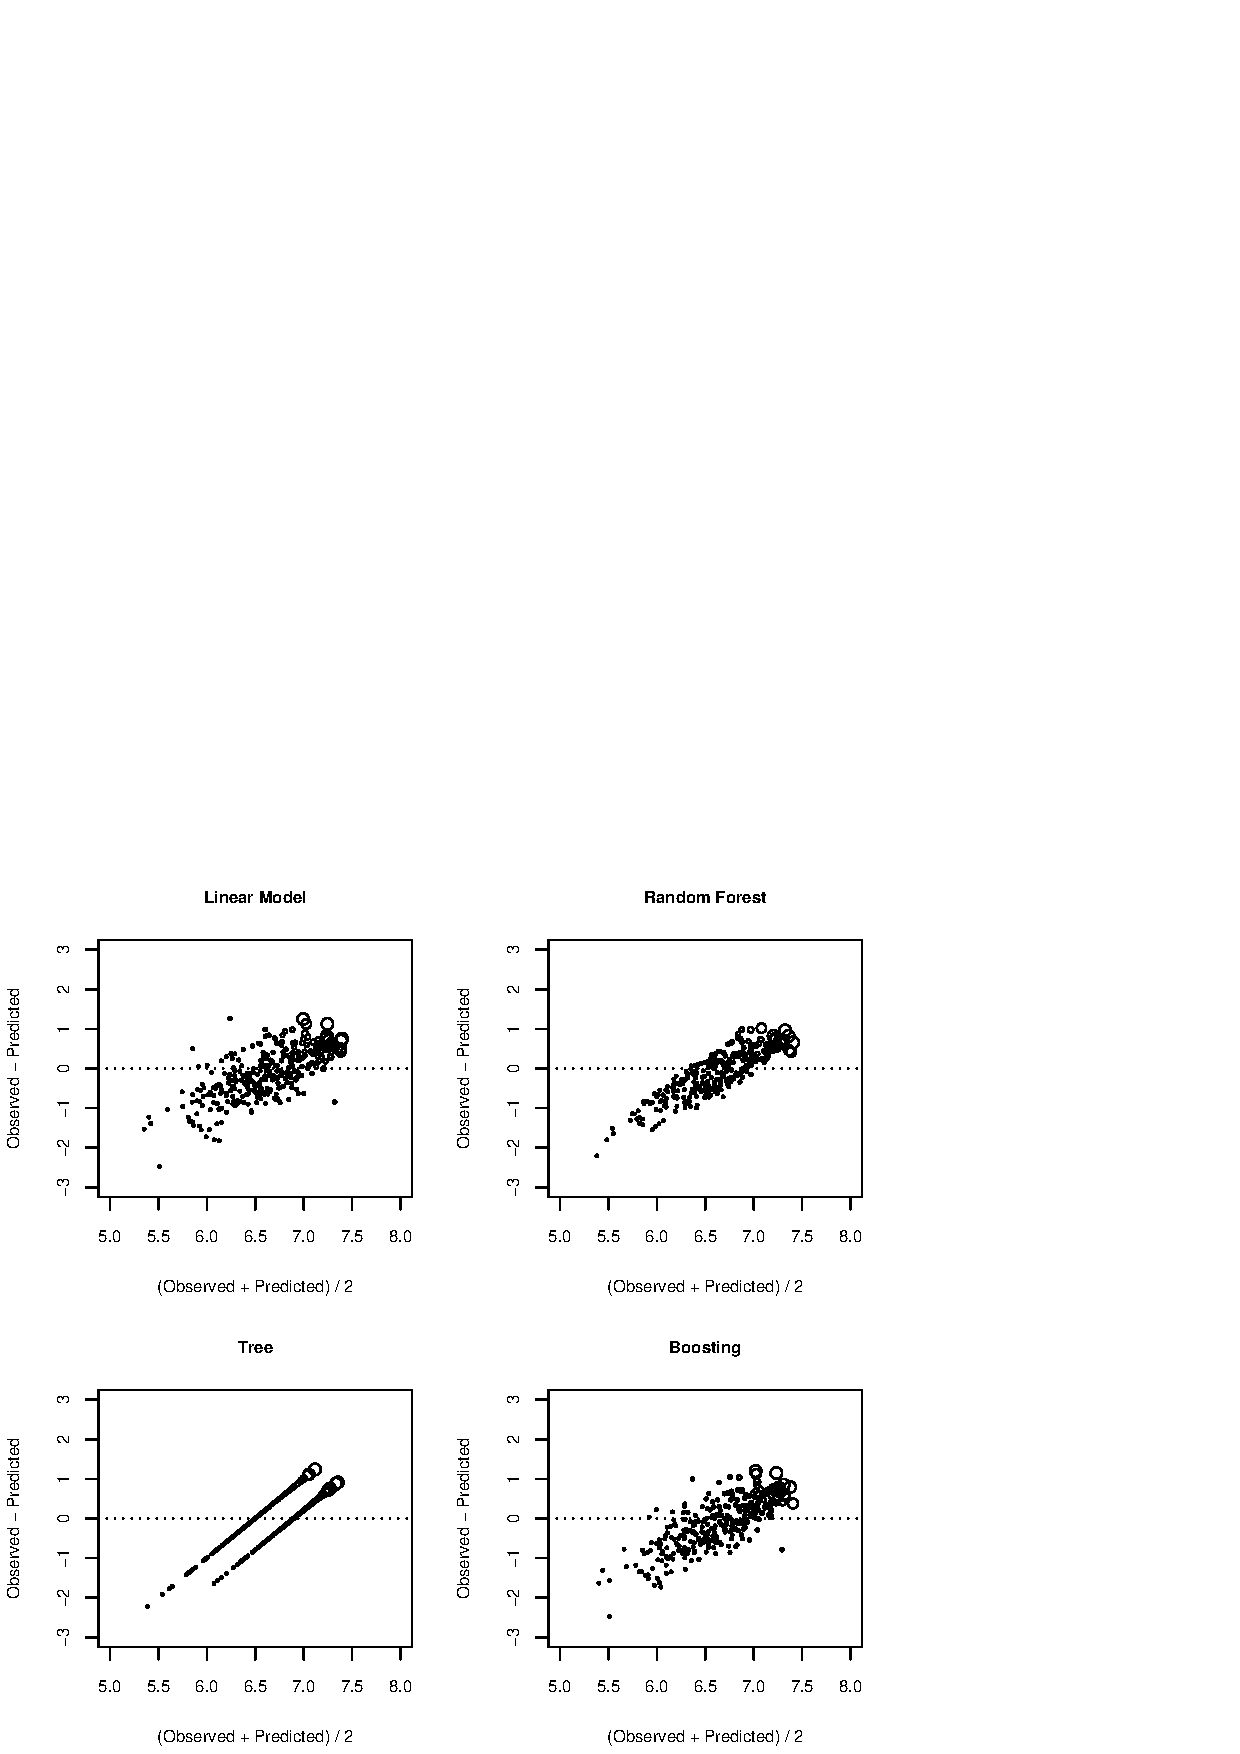
\includegraphics{SurvivalEnsembles-Figure3}
\caption{GBSG-2 data: Reproduction of Figure 3.}
\end{center}
\end{figure}

\begin{figure}
\begin{center}
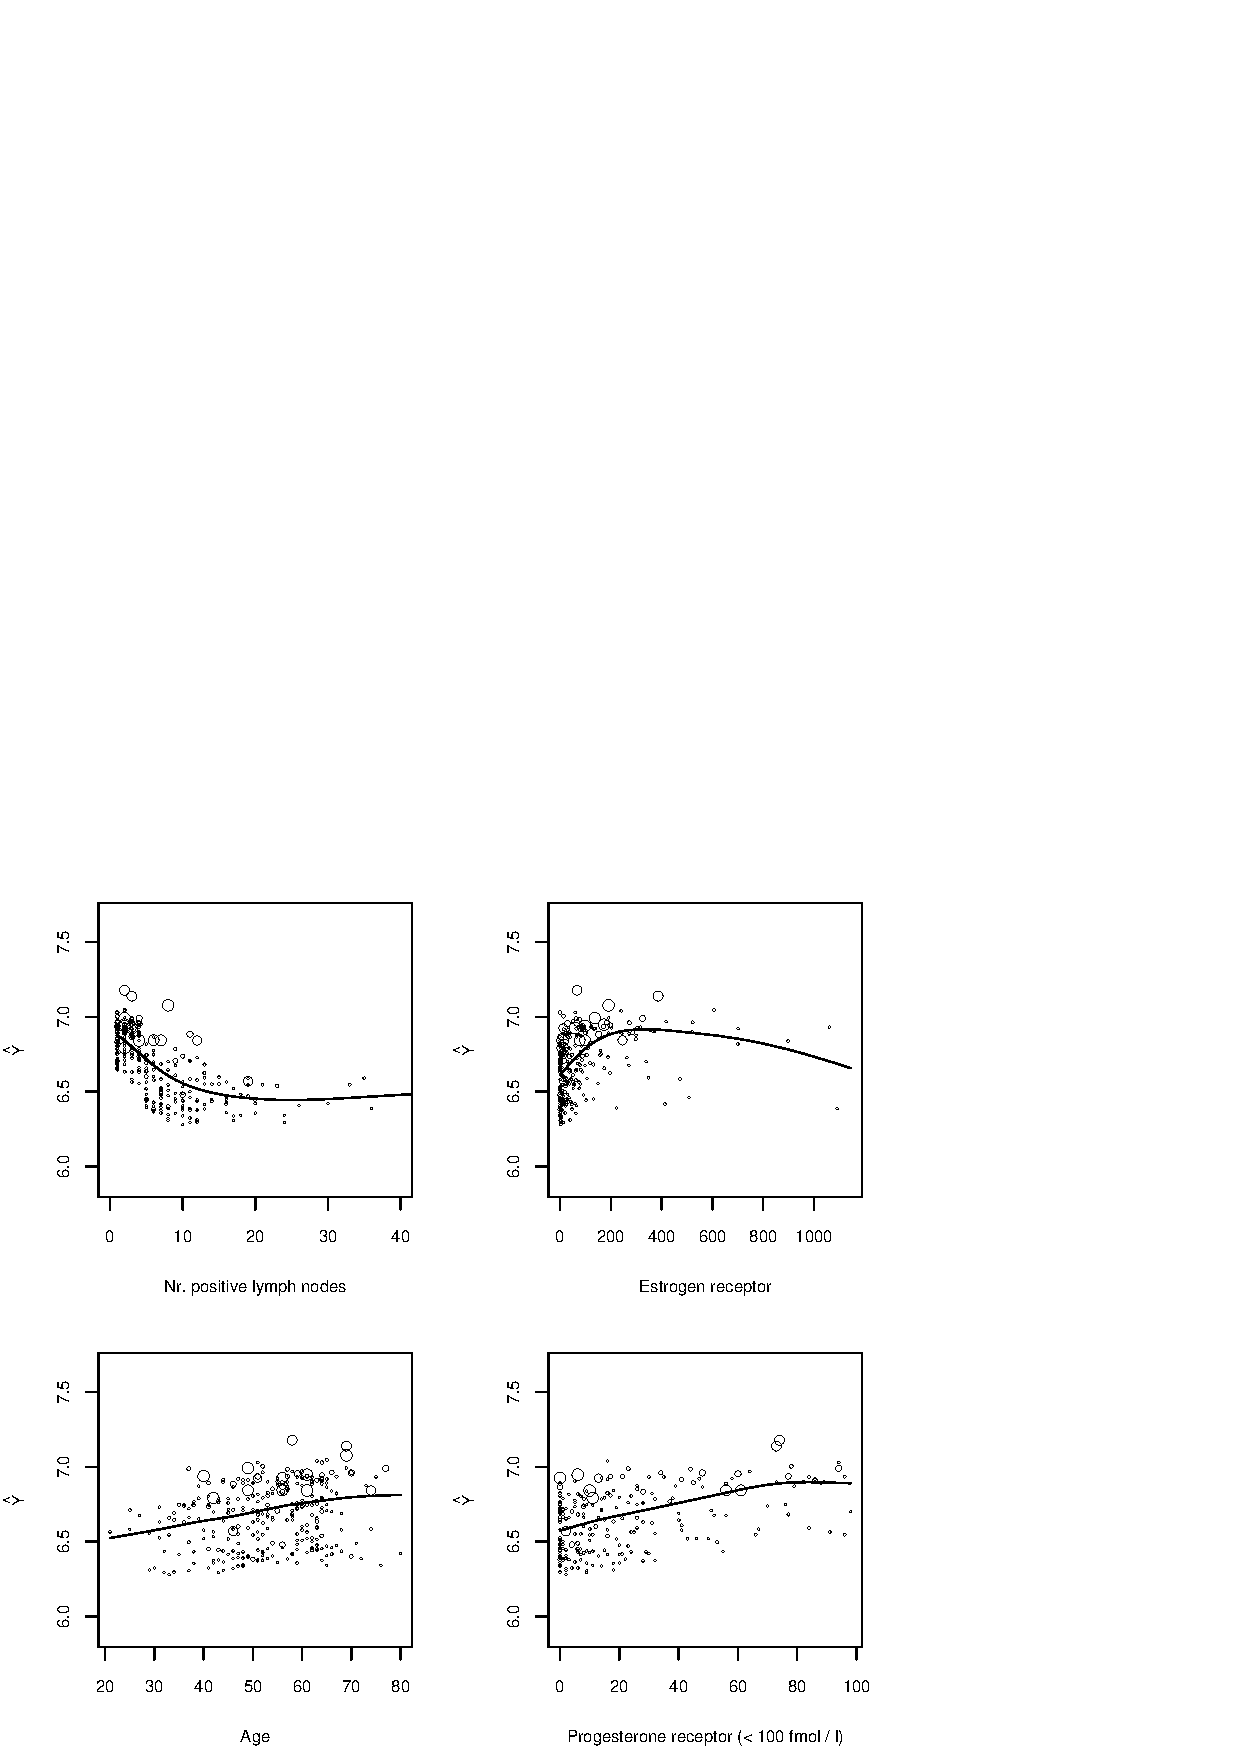
\includegraphics{SurvivalEnsembles-Figure5}
\caption{GBSG-2 data: Reproduction of Figure 5.}
\end{center}
\end{figure}


\begin{figure}
\begin{center}
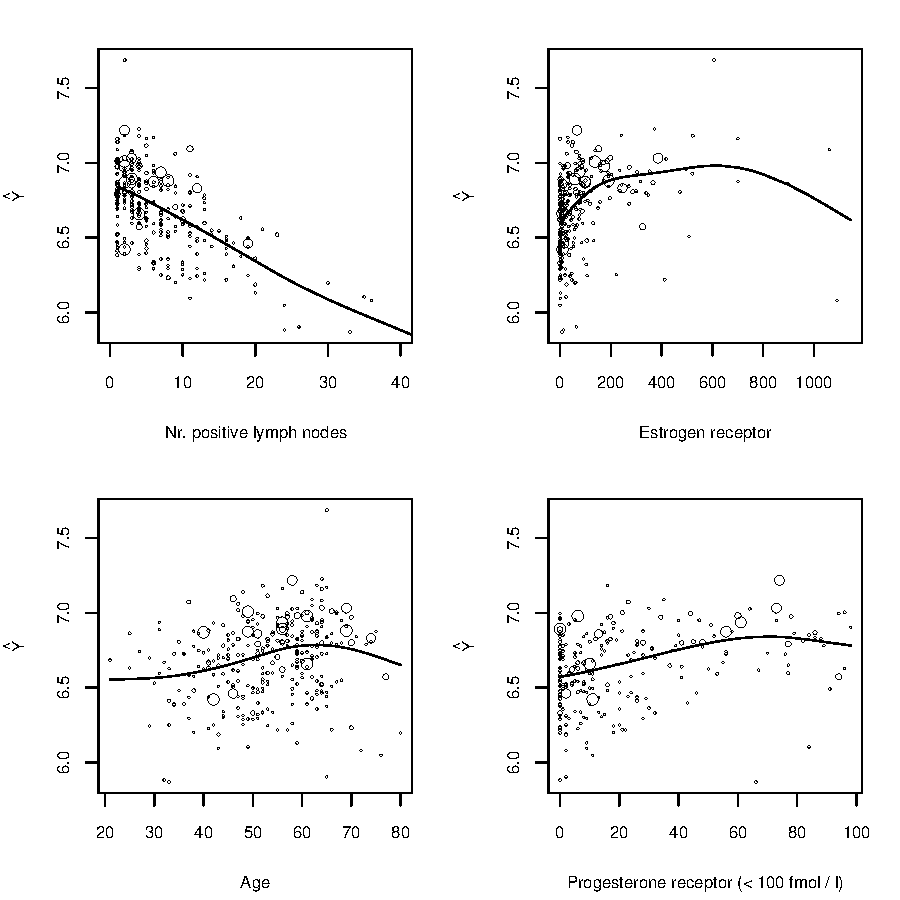
\includegraphics{SurvivalEnsembles-Figure6}
\caption{GBSG-2 data: Reproduction of Figure 6.}
\end{center}
\end{figure}

\begin{figure}
\begin{center}
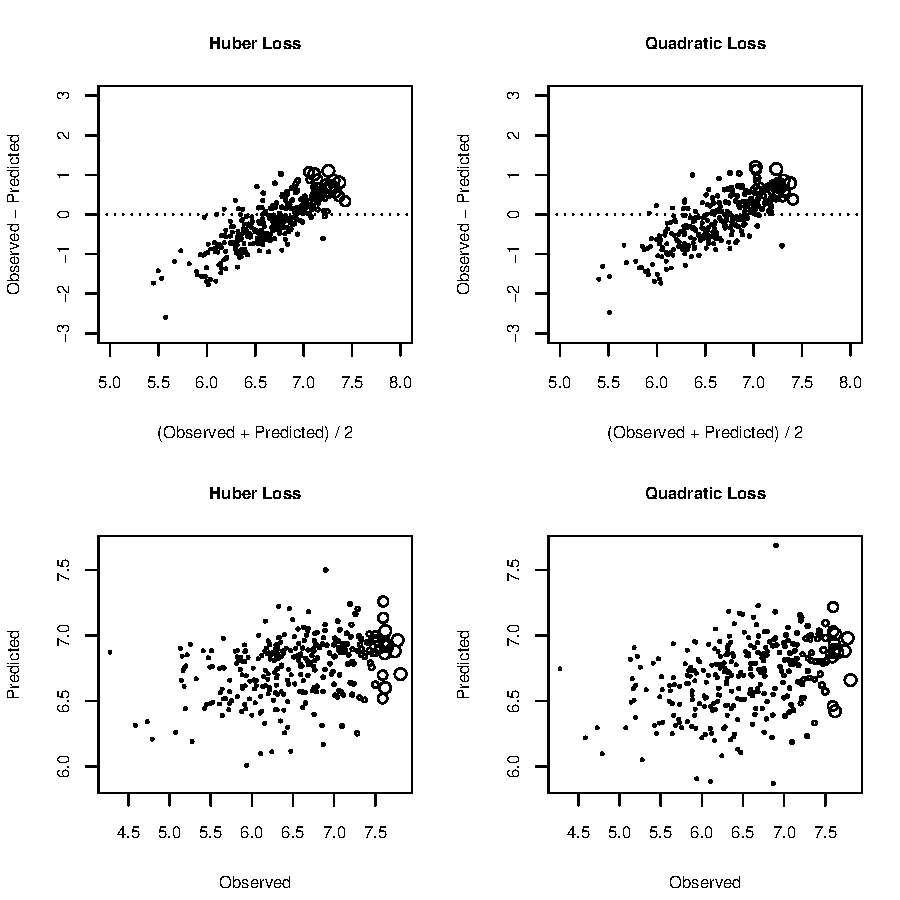
\includegraphics{SurvivalEnsembles-Figure7}
\caption{GBSG-2 data: Reproduction of Figure 7.}
\end{center}
\end{figure}

\clearpage

\bibliographystyle{plainnat}
\bibliography{boost}


\end{document}
